\usepackage{hyperref}
\usepackage{url}
\usepackage[margin=1in,marginpar=0.5in]{geometry} 
\usepackage{mathpazo_modified} 
\usepackage{amsmath}
\usepackage{calc} 
\usepackage{amssymb} 
\usepackage{amsthm} 
\usepackage{wrapfig} 
\usepackage{colonequals} 
\usepackage{ifthen}
\usepackage[labelfont=bf,labelsep=none,justification=RaggedRight]{caption}
\DeclareCaptionFormat{suggested}{{\small #1#2 #3}}
\captionsetup{format=suggested}
\usepackage{bm}

\newcommand{\milink}[3][-7.5mm]{  \sidenote{\href{http://mathinsight.org/#2}{\mi}
    on #3}[#1]}

\newcommand\cocalc[1][-2pt]{\raisebox{#1}{
\includegraphics[width=12pt]{figures/cocalc_new}}}
\newcommand\tbob[1][-2pt]{\raisebox{#1}{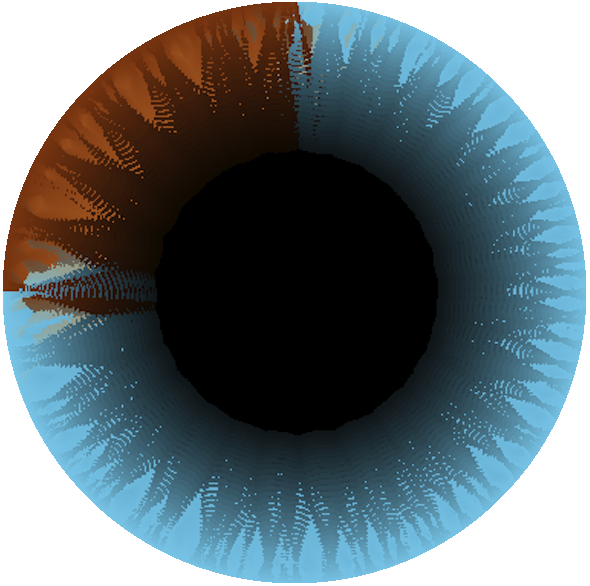
\includegraphics[width=12pt]{figures/3b1b_new}}}
\newcommand\mi[1][-2pt]{\raisebox{#1}{
\includegraphics[width=12pt]{figures/mathinsight}}}

\usepackage{array}
\newcolumntype{M}[1]{>{\centering\arraybackslash}m{#1}}
\newcolumntype{N}{@{}m{0pt}@{}}
\usepackage{multirow}

\newlength{\sidepanelwidth} 

\newcommand\twocol[2]{%
  \begin{minipage}{0.7\textwidth}
    \parskip = 0.2 in 
    #1
  \end{minipage} 
  \begin{minipage}{0.29\textwidth}
    #2
  \end{minipage}
}

\newcommand\twocolb[5]{%
  \begin{minipage}[#3]{#1\textwidth}
    \parskip = 0.2 in 
    #4
  \end{minipage} 
  \begin{minipage}[#3]{#2\textwidth}
    \raisebox{\dimexpr -\height + 1.5ex \relax}{#5}
  \end{minipage}
}

\DeclareMathOperator{\arcsec}{arcsec}
\DeclareMathOperator{\cis}{cis}
\DeclareMathOperator{\Real}{Re}
\DeclareMathOperator{\Imag}{Im}
\newcommand\cv[1]{\langle #1_1, #1_2, #1_3 \rangle}

\newcommand{\includebreaks}{true}
\newcommand{\forcebreak}{\ifthenelse{\equal{\includebreaks}{true}}{\newpage}{}}

\makeatletter                       
\def\printauthor{%                  
  {\large \@author}}              
\makeatother
\author{%
  {\Large \textit{Samuel S.\ Watson}} \\ \vspace{2mm}  sswatson@mit.edu
}

\numberwithin{equation}{section}

\usepackage[skins,theorems,breakable,raster]{tcolorbox}

\definecolor{softblue}{rgb}{0.92, 0.95, 0.99}
\definecolor{softyellow}{rgb}{0.98, 0.98, 0.9}
\definecolor{softseagreen}{rgb}{0.96, 0.995, 0.98}
\definecolor{softred}{rgb}{0.99, 0.92, 0.91}
\definecolor{softbrown}{rgb}{0.97, 0.97, 0.9}

\newtcbtheorem[number within=section]{theo}{Theorem}{colback=softred,colframe=red!35!black,fonttitle=\bfseries}{th}

\newtcbtheorem[number within=section]{obs}{Observation}{colback=Turquoise!8!white, colframe=Turquoise!50!black,fonttitle=\bfseries}{obs}

\newtcbtheorem[number
within=section]{exercise}{Exercise}{colback=softseagreen,colframe=SeaGreen,fonttitle=\bfseries,parbox=false}{exer}

\newtcbtheorem[number
within=section]{example}{Example}{enhanced, colback=softblue,colframe=MidnightBlue,fonttitle=\bfseries}{exam}


\newtcolorbox{solution}[1][title=Solution]{
  enhanced,
  breakable,
  parbox=false, 
  colback=softyellow,
  colframe=Orange!75!black,
  fonttitle=\bfseries,
  #1}


\newtcbtheorem{defn}{Definition}{colback=Purple!5,colframe=Purple,fonttitle=\bfseries}{defn}

\usepackage{tikz} 

%\usepackage[dvipsnames]{xcolor} 

\usepackage[explicit,calcwidth]{titlesec}
\newcommand*\chapterlabel{}
\titleformat{\chapter}
  {\gdef\chapterlabel{}
   \normalfont\sffamily\Huge\bfseries\scshape}
  {\gdef\chapterlabel{\thechapter\ }}{0pt}
  {\begin{tikzpicture}[remember picture,overlay]
    \node[yshift=-3cm] at (current page.north west)
      {\begin{tikzpicture}[remember picture, overlay]
        \draw[fill=softblue] (0,0) rectangle
          (\paperwidth,3cm);
        \node[anchor=east,xshift=.9\paperwidth,rectangle,
              rounded corners=20pt,inner sep=11pt,
              fill=MidnightBlue]
              {\color{white}\chapterlabel#1};
       \end{tikzpicture}
      };
   \end{tikzpicture}
  }
\titlespacing*{\chapter}{0pt}{50pt}{-60pt}

\titleformat{\section}
  {\addtolength{\titlewidth}{2pc}\normalfont\Large\sffamily\bfseries}
  {\colorbox{MidnightBlue}{\parbox{2cm}{\strut\color{white}\hfill\thesection}}}
  {1em}{#1}
  [{\titleline*[l]{\color{MidnightBlue}\titlerule[2pt]}}]
\titleformat{\subsection}
  {\addtolength{\titlewidth}{2pc}\normalfont\large\sffamily}
  {\colorbox{MidnightBlue}{\parbox{2cm}{\strut\color{white}\hfill\thesubsection}}}
  {1em}{#1}
  [{\titleline*[l]{\color{MidnightBlue}\titlerule[2pt]}}]


\usepackage{xparse} 
\usepackage{calc} 

\newlength{\marginvoffset} 

\newcounter{intld}
	\setcounter{intld}{0}

\newcounter{comp}
	\setcounter{comp}{0}

\newcounter{prob}
	\setcounter{prob}{1}

\newcounter{subitm}
        \setcounter{subitm}{1}

\usepackage{enumitem} 
\usepackage{marginnote} 

\setenumerate{labelsep=3pt,itemsep=0pt,parsep=0pt,topsep=0pt}
\setitemize{labelsep=3pt,itemsep=0pt,parsep=0pt,topsep=0pt}

\newcommand\subitm{(\alph{subitm})\quad\stepcounter{subitm}}

\newcommand{\pairofprobs}[2]{\makebox[0.5\textwidth][l]{\subitm #1}\subitm #2}

\usepackage[T1]{fontenc}
\usepackage[scaled=0.8]{beramono}

\usepackage{listings}
\definecolor{shadecolor}{rgb}{0.92,0.92,0.92}
\lstset{%
    language         = python,
    basicstyle       = \ttfamily,
    keywordstyle     = \bfseries\color{blue},
    stringstyle      = \color{magenta},
    commentstyle     = \color{ForestGreen},
    showstringspaces = false,
    backgroundcolor  = \color{shadecolor},
    belowskip        = -3mm
}

\let\oldmarginpar\marginpar
% renew the \marginpar command to draw 
% a node; it has a default setting which 
% can be overwritten
\renewcommand{\marginpar}[3][rectangle,text width = 1.75cm,draw,fill=blue!25,rounded corners]{%
        \oldmarginpar{%
          \hphantom{a} \vspace{#2}
        \scriptsize \tikz \node at (0,-1) [#1]{#3};
      }%
        }

\DeclareDocumentCommand{\sidenote}{O{rectangle,text width =
    17.5mm,draw,fill=softblue,rounded corners} m O{0pt}}{
       \setlength{\marginvoffset}{#3 - 12pt} 
        \marginnote[{%
          \makebox[0pt][r]{
            \scriptsize \tikz \node at (0,-1) [#1]{#2};
          }
          }]{}[\marginvoffset]%
}

\newcommand{\bang}[1]{\marginnote{ \Huge \color{DarkRed} !!!}[#1]}


\newcommand{\datemarker}[1]{\sidenote[rectangle,text width =
  1.75cm,draw,fill=black!25,rounded corners]{\centerline{#1}}}

\usepackage{color}
\definecolor{dg}{RGB}{2,101,15}
\definecolor{dr}{RGB}{80,15,40}

%This cover art is taken from 
%http://tex.stackexchange.com/questions/85904/showcase-of-beautiful-title-page-done-in-tex

\definecolor{titlepagecolor}{cmyk}{1,.60,0,.40}

\newcommand\titlepagedecoration{%
\begin{tikzpicture}[remember picture,overlay,shorten >= -10pt]

\coordinate (aux1) at ([yshift=-15pt]current page.north east);
\coordinate (aux2) at ([yshift=-410pt]current page.north east);
\coordinate (aux3) at ([xshift=-4.5cm]current page.north east);
\coordinate (aux4) at ([yshift=-150pt]current page.north east);

\begin{scope}[titlepagecolor!40,line width=12pt,rounded corners=12pt]
\draw
  (aux1) -- coordinate (a)
  ++(225:5) --
  ++(-45:5.1) coordinate (b);
\draw[shorten <= -10pt]
  (aux3) --
  (a) --
  (aux1);
\draw[opacity=0.6,titlepagecolor,shorten <= -10pt]
  (b) --
  ++(225:2.2) --
  ++(-45:2.2);
\end{scope}
\draw[titlepagecolor,line width=8pt,rounded corners=8pt,shorten <= -10pt]
  (aux4) --
  ++(225:0.8) --
  ++(-45:0.8);
\begin{scope}[titlepagecolor!70,line width=6pt,rounded corners=8pt]
\draw[shorten <= -10pt]
  (aux2) --
  ++(225:3) coordinate[pos=0.45] (c) --
  ++(-45:3.1);
\draw
  (aux2) --
  (c) --
  ++(135:2.5) --
  ++(45:2.5) --
  ++(-45:2.5) coordinate[pos=0.3] (d);   
\draw 
  (d) -- +(45:1);
\end{scope}
\end{tikzpicture}%
}


\parindent = 0.0 in
\parskip = 0.2 in 

\newcommand{\R}{\mathbb{R}}
\newcommand{\C}{\mathbb{C}}
\newcommand{\Z}{\mathbb{Z}}

\DeclareFixedFont{\titlefont}{T1}{ppl}{b}{it}{0.4in}
\DeclareFixedFont{\subtitlefont}{T1}{ppl}{b}{it}{12pt}

\usepackage{asymptote}

\begin{asydef} 
defaultpen(fontsize(10));
settings.outformat="pdf";
usepackage("mathpazo_modified");
import x11colors;
pen softblue = rgb(0.92,0.95,0.99);
pen softred = rgb(0.99, 0.92, 0.91);
pen softyellow = rgb(0.98, 0.98, 0.9);
pen softgreen = rgb(0.96, 0.995, 0.98);
settings.render = 8; 
\end{asydef}

%----CUSTOMIZE TABLE OF CONTENTS SPACING -------
\usepackage{tocloft}
\renewcommand\cftchapafterpnum{\vskip5pt}
\renewcommand\cftsecafterpnum{\vskip5pt}
\renewcommand\cftsubsecafterpnum{\vskip5pt}

\newsavebox{\asybox}
\def\asydir{asy}